\documentclass{beamer}

\usepackage{amsmath}
\usepackage{amssymb}
\usepackage{sfmath}
\usepackage{cmbright}
\usepackage{cancel}

%Information to be included in the title page:
\title{Spacecraft Motion with Thrust Normal to Velocity Vector}
\date{June 15-29 2021}

\begin{document}

\frame{\titlepage}

\begin{frame}

\frametitle{Weekly Progress}

\begin{itemize}
    \item June 10-15
    \begin{itemize}
        \item Found expression for $w_1(\phi)$ from $w(r)$ in terms of $\phi$ and $\beta$
        \item Found an expression for $y_1(\phi)$ given $y(r)$
        \item Found discrepancy between plots of $w(r)$ and $w_1(\phi)$ using Desmos and Octave
    \end{itemize}
    \item June 15-29
    \begin{itemize}
        \item Checked work for $w_1(\phi)$ and adjusted expression to account for newly provided definition of $\beta$
        \item Found an expression for $y_1(\phi)$ given $y(r)$ using new definition
        \item Numerically minimized $w_1(\phi)$ after obtaining a complicated relation (simplified to best means)
        \item Work was checked thoroughly using Desmos and Octave plots
    \end{itemize}
\end{itemize}

\end{frame}

\begin{frame}
    \frametitle{Expressing $w(r)$ in terms of $\phi$ and $\beta$}

    Approach: reexpress components of $w(r)$ and substitute $r(\phi)$

    
    {\scriptsize{$$
    w(r)=\underbrace{\frac{r_{0}}{\sqrt{r\left(2 r_{0}-r\right)}}}_{w_1(r)}
        \underbrace{\left[1-\frac{a_{T} r_{0}^{2}}{\mu}\left(3 \sin ^{-1}\left(\sqrt{\frac{r}{2 r_{0}}}\right)-\frac{3 \pi}{4}+2\right)\right]}_{w_2(r)}
        +\underbrace{\frac{a_{T} r_{0}}{2 \mu}\left(r+3 r_{0}\right)}_{w_3(r)}
    $$}}

    For plots: $r_0=1, \mu=1, a_T=0.2$\newline
    Definitions: $k(\phi)=\phi+\pi/4$, $r(\phi)=2r_0\sin^2(k)$, $\beta=\sqrt{\frac{4\mu}{(3\pi+8)a_Tr_0^2}}$\newline
    Subscript $p$ denotes function of $\phi$.

\end{frame}

\begin{frame}
    \frametitle{Plotting $w_1(r),w_2(r),w_3(r)$}

    \begin{center}
        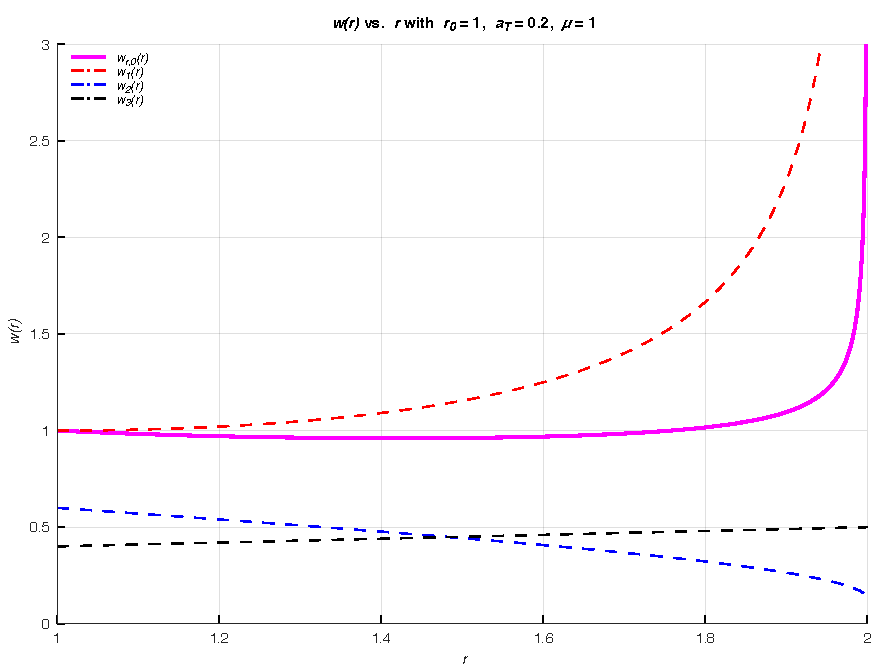
\includegraphics[scale=0.7]{plots/partA_r.pdf}
    \end{center}
\end{frame}

\begin{frame}
    \frametitle{Reexpressing $w_1(r)$}

    \begin{align}
        w_{1p}(\phi)&=\frac{r_{0}}{\sqrt{r\left(2 r_{0}-r\right)}}_{\big\rvert_{r(\phi)}}\\
        &=\frac{r_0}{\sqrt{2r_0\sin^2(k)(2r_0-2r_0\sin^2(k))}}\\
        &=\frac{r_0}{\sqrt{4r_0^2\sin^2(k)\cos^2(k)}}\\
        &=\frac{1}{\sin(2k)}
    \end{align}

    Obtain 3 using $\cos^2(k)=1-\sin^2(k)$ and 4 by $\sin(2k)=2\sin(k)\cos(k)$.
    
\end{frame}

\begin{frame}
    \frametitle{Reexpressing $w_2(r)$}

    \begin{align}
        w_{2p}(\phi)&=1-\frac{a_Tr_0^2}{\mu}\left(3\arcsin(\sqrt{\frac{r}{2r_0}})-\frac{3\pi}{4}+2\right)_{\big\rvert_{r(\phi)}}\\
        &=1-\frac{a_Tr_0^2}{\mu}\underbrace{\left(3k-\frac{3\pi}{4}+2\right)}_{3\phi + 2}\\
        &=1-\frac{a_Tr_0^2}{\mu}\left(3\phi+2\right)
    \end{align}
\end{frame}

\begin{frame}
    \frametitle{Reexpressing $w_3(r)$}

    \begin{align}
        w_{3p}(\phi)&=\frac{a_Tr_0}{2\mu}(r+3r_0)_{\big\rvert_{r(\phi)}}\\
        &=\frac{a_Tr_0}{2\mu}(r_0(2\sin^2(k)+3))\\
        &=\frac{a_Tr_0^2}{2\mu}(2\sin^2(k)+3)\\
        &=\frac{2}{\beta^2(3\pi+8)}(2\sin^2(k)+3)
    \end{align}

    Obtain 11 by $\beta=\sqrt{\frac{4\mu}{(3\pi+8)a_Tr_0^2}}\implies \frac{1}{\beta^2}=\frac{(3\pi+8)a_Tr_0^2}{4\mu}$
\end{frame}

\begin{frame}
    \frametitle{Expression for $w_p(\phi)$}

    \begin{align}
        w_p(\phi)&=\frac{1}{\sin(2k)}\left[1-\frac{a_Tr_0^2}{\mu}\left(3\phi+2\right)\right]\frac{2}{\beta^2(3\pi+8)}(2\sin^2(k)+3)\\
        &=w_{1p}(\phi)w_{2p}(\phi)+w_{3p}(\phi)
    \end{align}
\end{frame}

\begin{frame}
    \frametitle{Checking answer with plots}

    \begin{center}
        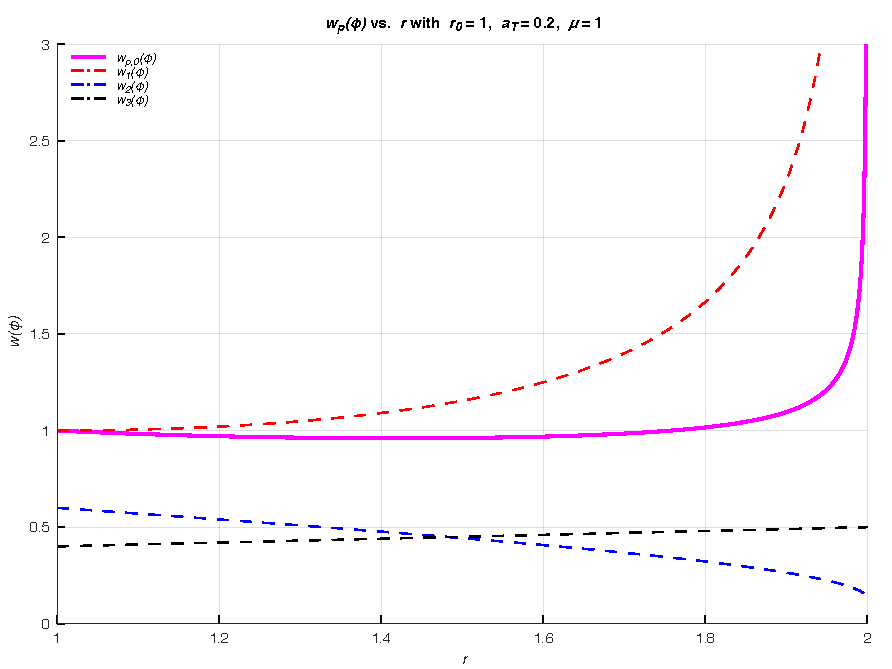
\includegraphics[scale=0.7]{plots/partA_phi.pdf}
    \end{center}
\end{frame}

\begin{frame}
    \frametitle{Expressing $y(r)$ in terms of $\phi$ and $\beta$}

    Approach similar to $w(r)$:
    $$
    y(r)=\underbrace{\sqrt{\frac{\mu(2r_0-r)}{rr_0}}}_{y_1(r)}\underbrace{\sqrt{1-w(r)^2}}_{y_2(r)}
    $$
\end{frame}

\begin{frame}
    \frametitle{Reexpressing $y_1(r)$}

    \begin{align}
        y_{1p}(\phi)&=\sqrt{\frac{\mu(2r_0-r)}{rr_0}}\bigg\rvert_{r(\phi)}\\
        &=\sqrt{\frac{\mu 2r_0(1-\cos^2(k))}{2r_0^2\sin^2(k)}}\\
        &=\sqrt{\frac{\mu 2r_0 \cos^2(k)}{2r_0^2 \sin^2(k)}}\\
        &=\sqrt{\frac{\mu}{r_0}}\cot(k)
    \end{align}
\end{frame}

\begin{frame}
    \frametitle{Reexpressing $y_2(r)$}

    Given $y_{2p}(\phi)=\sqrt{1-w_p(\phi)^2}$.\newline
    Define $\varphi(\phi)$ such that $\frac{\varphi(\phi)}{(3\pi+8)^2\beta^4\sin^2(2k)}=1-w_p(\phi)^2$.

    Then, by squaring 12,

    {\tiny
        \begin{align*}
            1-w_p(\phi)^2&=\frac{(3\pi+8)^2\beta^4\sin^2(2k)-\left[(3\pi+8)^2\beta^4-8(3\phi+2)(3\pi+8)\beta^2+16(3\phi+2)^2\right]}{(3\pi+8)^2\beta^4\sin^2(2k)}\\
            &-\frac{2\sin(2k)(4\sin^2(k)+6)((3\pi+8)\beta^2-4(3\phi+2))}{(3\pi+8)^2\beta^4\sin^2(2k)}\\
            &-\frac{\sin^2(2k)(16\sin^4(k)+48\sin^2(k)+36)}{(3\pi+8)^2\beta^4\sin^2(2k)}
        \end{align*}
    }

    Extracting the denominator,

    $$
    y_p(\phi)=\frac{\sqrt{\varphi(\phi)}}{\beta^2(3\pi+8)\sin(2k)}\sqrt{\frac{\mu}{r_0}}\cot(k)
    $$

\end{frame}

\begin{frame}
    \frametitle{Plots to verify $y_p(\phi)$}

    \begin{center}
        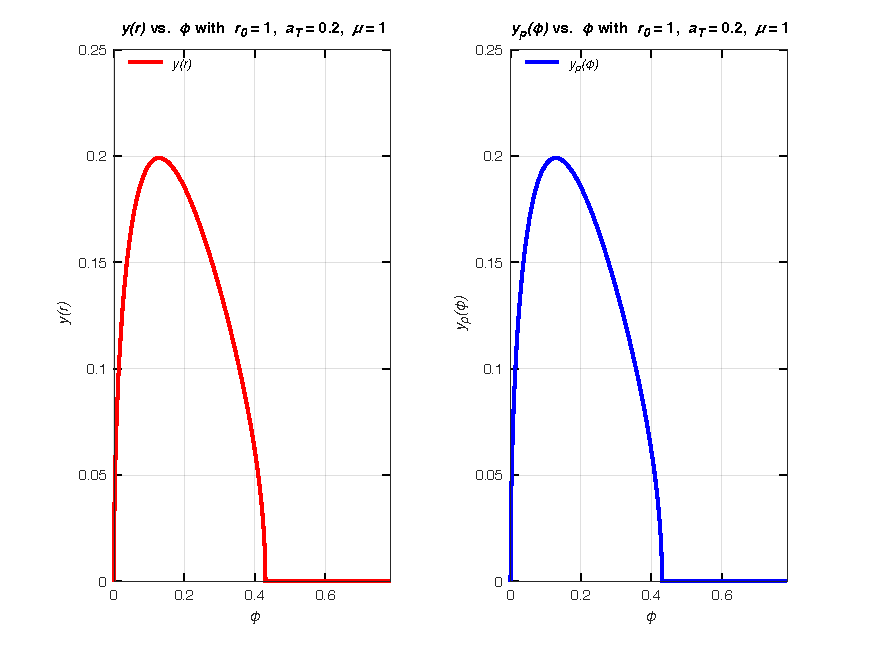
\includegraphics[scale=0.7]{plots/partB.pdf}
    \end{center}
\end{frame}

\begin{frame}
    \frametitle{Minimizing $w(r)$ or $w_p(\phi)$}

    \begin{itemize}
        \item Began by differentiating $w(r)$ and simplifying
        \item Substituted $r(\phi)$ to find $w_p\,'(\phi)$
        \item Solving for $\phi$ in $w_p\,'(\phi)$ would not be feasible by hand since there were trigonometric and linear terms of $\phi$
        \begin{itemize}
            \item Obtained a greatly simplified expression that was used for minimization
        \end{itemize}
        \item Used Octave to minimize the expression numerically
    \end{itemize}

\end{frame}

\begin{frame}
    \frametitle{First derivative test on $w(r)$}

    {\tiny\begin{align}
        w_1\,'(r)&=\frac{d}{dr}r_0(2r_0r-r^2)^{-1/2}\\
        &=-\frac{1}{2}r_0(2r_0-2r)(2r_0r-r^2)^{-3/2}\\
        &=\frac{-r_0(r_0-r)}{(2r_0r-r^2)^{3/2}}\\
        w_2\,'(r)&=\frac{-3a_Tr_0^2}{\mu}\frac{d}{dr}\arcsin \sqrt{\frac{r}{2r_0}}\\
        &=\frac{-3a_Tr_0^2}{\mu}\frac{\frac{1}{4r_0}(\frac{r}{2r_0})^{-\frac{1}{2}}}{\sqrt{1-\frac{r}{2r_0}}}\\
        &=\frac{-3a_Tr_0}{\mu}\frac{1}{4\sqrt{\frac{r}{2r_0}(\frac{2r_0-r}{2r_0})}}\\
        &=-\frac{3a_Tr_0}{2\mu\sqrt{2r_0r-r^2}}\\
        w_3\,'(r)&=\frac{d}{dr}\frac{a_Tr_0}{2\mu}(r+3r_0)\\
        &=\frac{a_Tr_0}{2\mu}
    \end{align}}
\end{frame}

\begin{frame}
    \frametitle{First derivative test on $w(r)$ (continued)}

    \begin{align}
        w\,'(r)&=\frac{d}{dr}\left[w_1(r)w_2(r)+w_3(r)\right]\\
        &=w_1\,'(r)w_2(r)+w_1(r)w_2\,'(r)+w_3\,'(r)
    \end{align}

    Substituting expressions found prior,

    {\scriptsize\begin{align}
        w\,'(r)&=\underbrace{\frac{-r_0(r_0-r)}{(2r_0r-r^2)^{3/2}}}_{w_1\,'(r)}\underbrace{\left[1-\frac{a_Tr_0^2}{\mu}\left(3\arcsin(\sqrt{\frac{r}{2r_0}})-\frac{3\pi}{4}+2\right)\right]}_{w_2(r)}\\
        &\underbrace{-\frac{3a_Tr_{0}}{2\mu\left(2 r_{0}r-r^2\right)}}_{w_1(r)w_2\,'(r)}+\underbrace{\frac{a_Tr_0}{2\mu}}_{w_3(r)}
    \end{align}}

\end{frame}

\begin{frame}
    \frametitle{Reubstituting with $r(\phi)$ and simplifying}

    First, $2r_0r-r^2=4r_0^2\sin^2(k)-4r_0sin^4(k)=4r_0^2\sin^2(k)\cos^2(k)$.

    {\begin{align}
        w_{1p}\,'(\phi)&=\frac{2r_0^2\sin^2(k)-r_0^2}{\left(2r_0\sin(k)\cos(k)\right)^3}=\frac{2\sin^2(k)-1}{r_0\sin^3(2k)}\\
        w_{2p}(\phi)&=1-\frac{a_Tr_0^2}{\mu}(3\phi+2)\\
        w_1(r)w_2\,'(r)&=-\frac{3a_Tr_0}{2\mu(4r_0^2\sin^2(k)\cos^2(k))}=-\frac{3a_Tr_0}{2\mu\sin^2(2k)}
    \end{align}}

    Then, 
    {\footnotesize\begin{equation}
        w_p\,'(\phi)=\frac{2\sin^2(k)-1}{r_0\sin^3(2k)}\left(1-\frac{a_Tr_0^2}{\mu}(3\phi+2)\right)-\frac{3a_Tr_0}{2\mu\sin^2(2k)}+\frac{a_Tr_0}{2\mu}
    \end{equation}}

\end{frame}

\begin{frame}
    \frametitle{Reubstituting with $r(\phi)$ and simplifying (continued)}

    {\footnotesize\begin{align}
        w_p\,'(\phi)&=\underbrace{\frac{2\sin^2(k)-1}{r_0\sin^3(2k)}\left(1-\frac{a_Tr_0^2}{\mu}(3\phi+2)\right)}_{\frac{-2\mu\cos(2k)\left(1-\frac{a_Tr_0^2}{\mu}(3\phi+2)\right)}{2\mu r_0\sin^3(2k)}}\underbrace{-\frac{3a_Tr_0}{2\mu\sin^2(2k)}+\frac{a_Tr_0}{2\mu}}_{\frac{a_Tr_0^2\sin^3(2k)-3a_Tr_0^2\sin(2k)}{2\mu r_0\sin^3(2k)}}\\
        &=\frac{a_Tr_0^2\left(\sin^3(2k)-3\right)\sin(2k)-2\mu\cos(2k)\left(1-\frac{a_Tr_0^2}{\mu}(3\phi+2)\right)}{2\mu r_0\sin^3(2k)}
    \end{align}}
\end{frame}

\begin{frame}
    \frametitle{Minimization of $w_p(\phi)$}

    Note that $2\mu r_0\sin^3(2k)\neq 0\implies \sin(2k)\neq 0$. So $2(\phi+\pi/4)\not\in \{0,\pi\}$ means $\phi\neq \pi/4$ since $\phi\in [0,\pi/4)$.

    {\scriptsize\begin{gather}
        w_p\,'(\phi)=\frac{a_Tr_0^2\left(\sin^3(2k)-3\right)\sin(2k)-2\mu\cos(2k)\left(1-\frac{a_Tr_0^2}{\mu}(3\phi+2)\right)}{2\mu r_0\sin^3(2k)}=0\\
        \implies a_Tr_0^2\left(\sin^3(2k)-3\right)\sin(2k)-2\mu\cos(2k)\left(1-\frac{a_Tr_0^2}{\mu}(3\phi+2)\right)=0\\
        \frac{\sin(2k)}{2\mu\cos(2k)}=\underbrace{\frac{\tan(2k)}{2\mu}}_{d_1(\phi)}=\underbrace{\frac{1-\frac{a_Tr_0^2}{\mu}(3\phi+2)}{a_Tr_0^2(\sin^3(2k)-3)}}_{d_2(\phi)}
    \end{gather}}

    Numerically finding the intersection of $d_1(\phi)$ and $d_2(\phi)$ yields the value of $\phi$ at $\text{min}(w_p(\phi))$, which can then be used to find $r$ for $\text{min}(w(r))$.

\end{frame}

\begin{frame}
    \frametitle{Numerical minimization of $w_p(\phi)$}
\end{frame}

\begin{frame}
    \frametitle{Intersection of $d_1(\phi)$ and $d_2(\phi)$}

    \begin{center}
        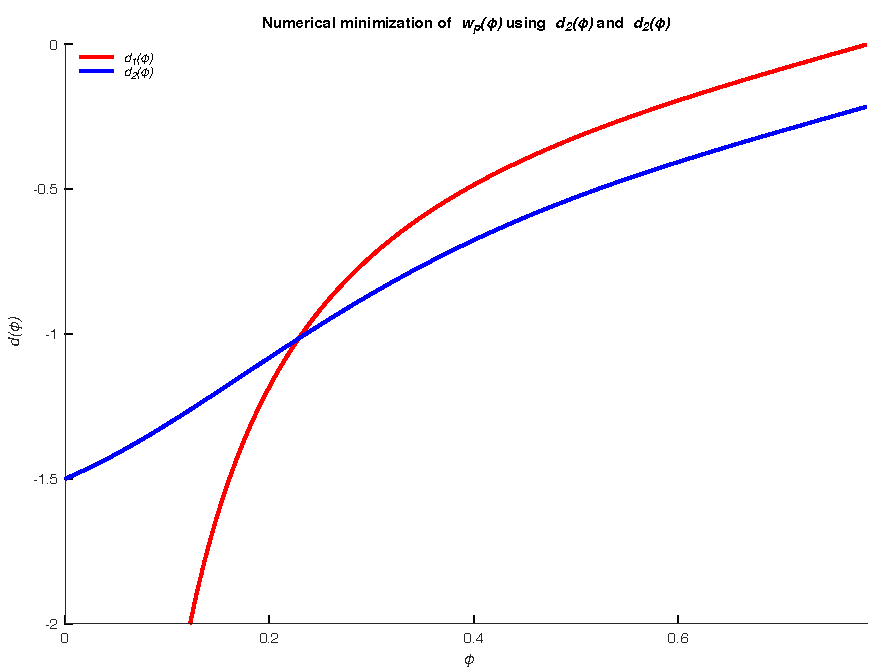
\includegraphics[scale=0.7]{plots/partC_min.pdf}
    \end{center}
\end{frame}

\begin{frame}
    \frametitle{Visual of $\text{min}(w_p(\phi))$}

    \begin{center}
        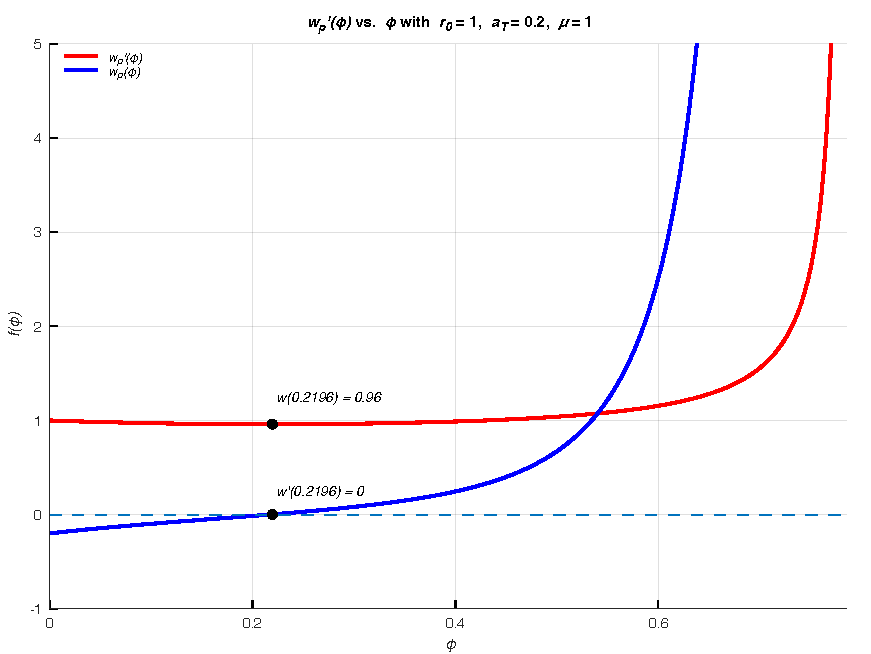
\includegraphics[scale=0.7]{plots/partC_r.pdf}
    \end{center}
\end{frame}

\end{document}